\chapter{Evaluation}\label{ch:evaluation}

\section{Evaluation Setup}
In order to evaluate the performance of our library, we measured the time required to upload, download and delete files which ranged from 1MB to 1GB in size. We executed all 3 operations on each file size, for each service (Dropbox, Box, Google Drive, S3), 5 times, and then calculated and recorded the mean duration. The specifications of the computer and network used to make the API calls and measure execution time are detailed in table \ref{tab:pc_specs}. Furthermore, chunked uploads were used across all services, with a chunk size of 32MB. The only exception to this was Box, as it automatically determined the optimal chunk size which was, however, 32MB for larger files ($>$100MB). Finally, no warm-up time was used for this evaluation.

\begin{table}[!h]
    \centering
    \begin{tabular}{|
            >{\columncolor[HTML]{EFEFEF}}l |l|}
        \hline
        \textbf{Operating System} & Windows 10                                      \\ \hline
        \textbf{Processor}        & Intel(R) Core(TM) i5-9600K CPU @ 3.70GHz        \\ \hline
        \textbf{Memory}           & 16GB RAM                                        \\ \hline
        \textbf{Storage}          & 1TB NVMe SSD                                    \\ \hline
        \textbf{Network}          & 100Mbps download and 10Mbps upload via Ethernet \\ \hline
    \end{tabular}
    \caption{PC and Network Specifications}
    \label{tab:pc_specs}
\end{table}

\section{Upload Duration}
The results on upload duration are depicted in figure \ref{fig:upload_duration} and \ref{fig:upload_log_duration}, and it can be observed that all services perform more or less identically for small file sizes (i.e. sizes smaller than 50MB). From that point on,  as the file sizes increase, S3 and Dropbox continue to exhibit very comparable performance, with upload times steadily increasing as the file size also increases.  However, Box and especially Google Drive struggle to keep up. Specifically, Box performs about as well as S3 and Dropbox for file sizes up to 100, but then starts to fall behind, requiring around 1 additional minute to complete the uploads. Google Drive fares much worse, though, as it performs quite well for small file sizes, but its performance starts to seriously degrade for 50MB files or larger. In fact, it requires around double the amount of time and, in some cases, even more than that. This poor performance can only be explained by limitations that have been placed which affect the  upload speed when making calls to the Google Drive API for chunked uploads of larger files. Regardless of the chunk size that was specified, no noticeable improvement was noticed, and this underwhelming performance of chunked uploads has been reported by other API users in the past ~\cite{drive_chunked_performance}. In general, from our evaluation, Amazon S3 was the fastest, with 457s for 1GB, while Box and Dropbox needed 538s and 483s, respectively, for the same file. Google Drive was by far the slowest, requiring 1154s for 1GB.

\begin{figure} []
    \centering
    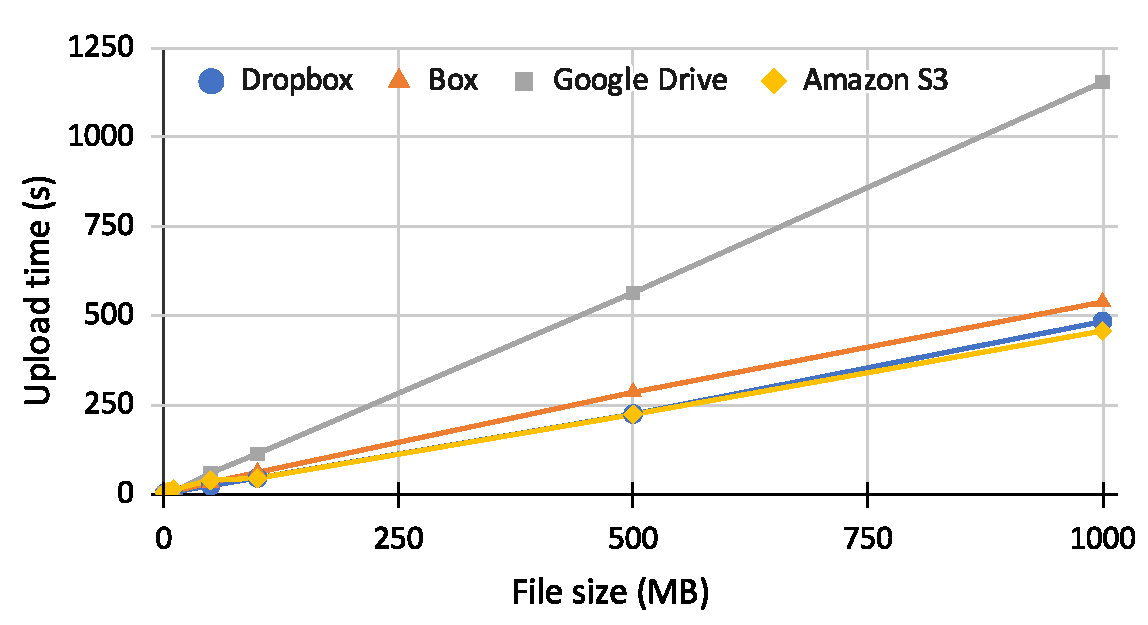
\includegraphics[scale=0.6]{images/upload_chart}
    \caption{\label{fig:upload_duration}Upload Duration}
\end{figure}

\begin{figure} [!h]
    \centering
    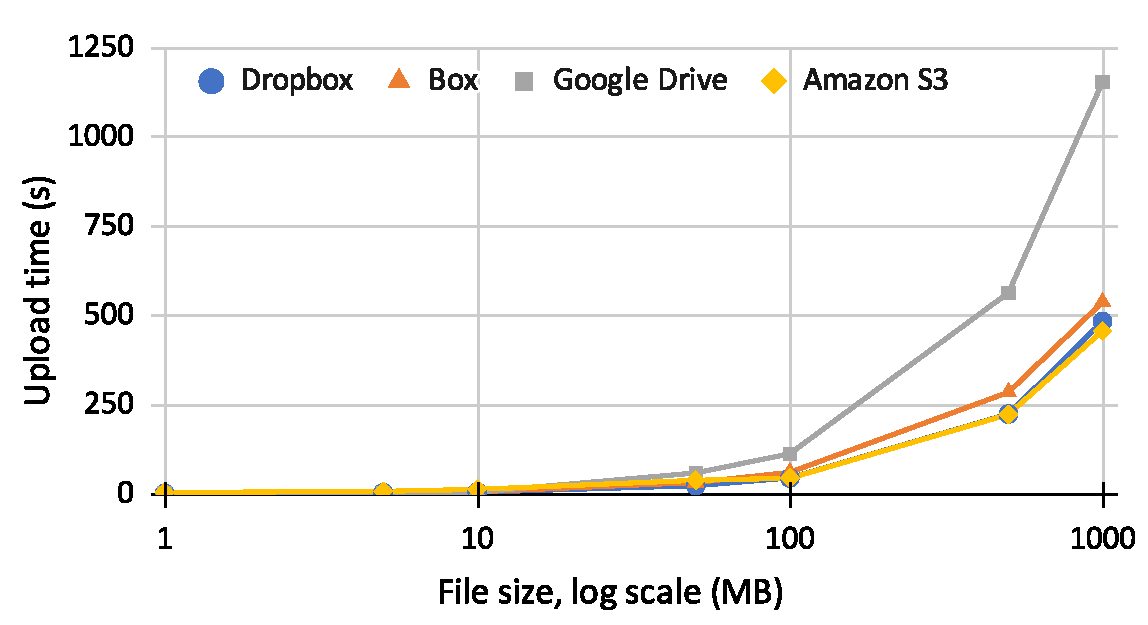
\includegraphics[scale=0.6]{images/upload_log_chart}
    \caption{\label{fig:upload_log_duration}Upload Duration (log scale)}
\end{figure}

\section{Download Duration}
As shown in figures \ref{fig:download_duration} and \ref{fig:download_log_duration}, the differences in download times aren't as significant. All services perform roughly the same for files that do not go over 100MB in size. However, among all the services, Dropbox is the fastest for small to medium sized files ($< 100$MB). For larger files ($ >$100MB), though, S3 takes the first place as it is consistently faster than Dropbox up until 1GB file size is reached, at which point both services achieve a roughly equal performance. The other two services (Box and Google Drive) are slower by 10-30s for files larger than 100MB. It is worth noting here that Google Drive was the only service which supported, and required, chunked downloads, but this didn't appear to cause any significant deviation in performance. Overall, S3 and Dropbox were the fastest when downloading, with 134s and 137s, respectively, for a 1GB file whereas Google Drive took 150s. Box was the slowest, with an upload speed of 162s for the same 1GB file.

\begin{figure} [!h]
    \centering
    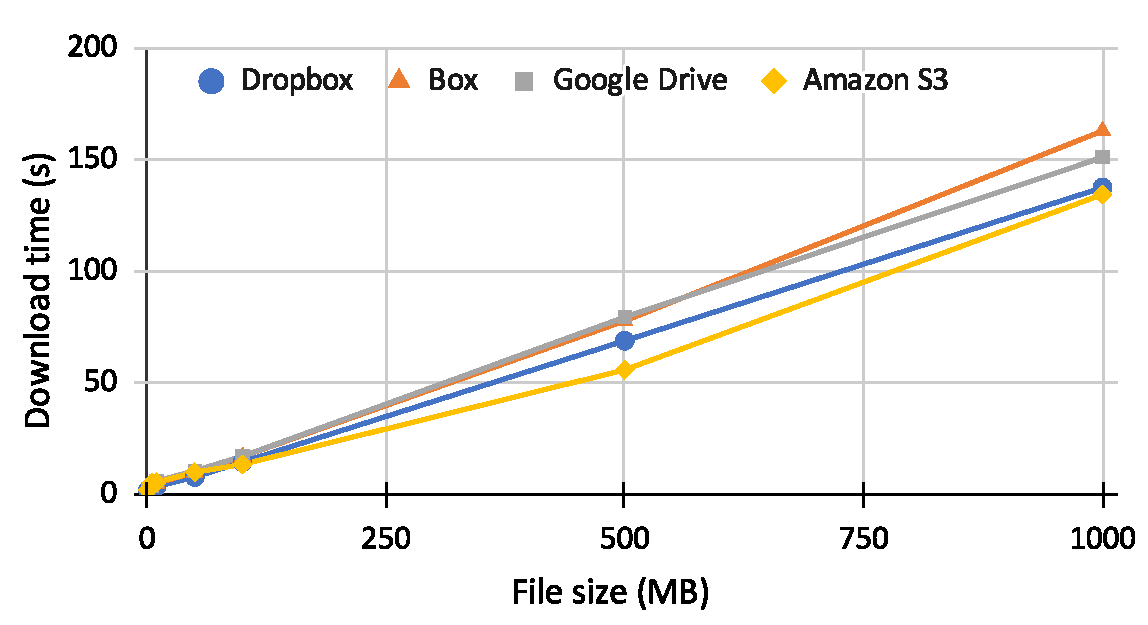
\includegraphics[scale=0.6]{images/download_chart}
    \caption{\label{fig:download_duration}Download Duration}
\end{figure}

\begin{figure} [!h]
    \centering
    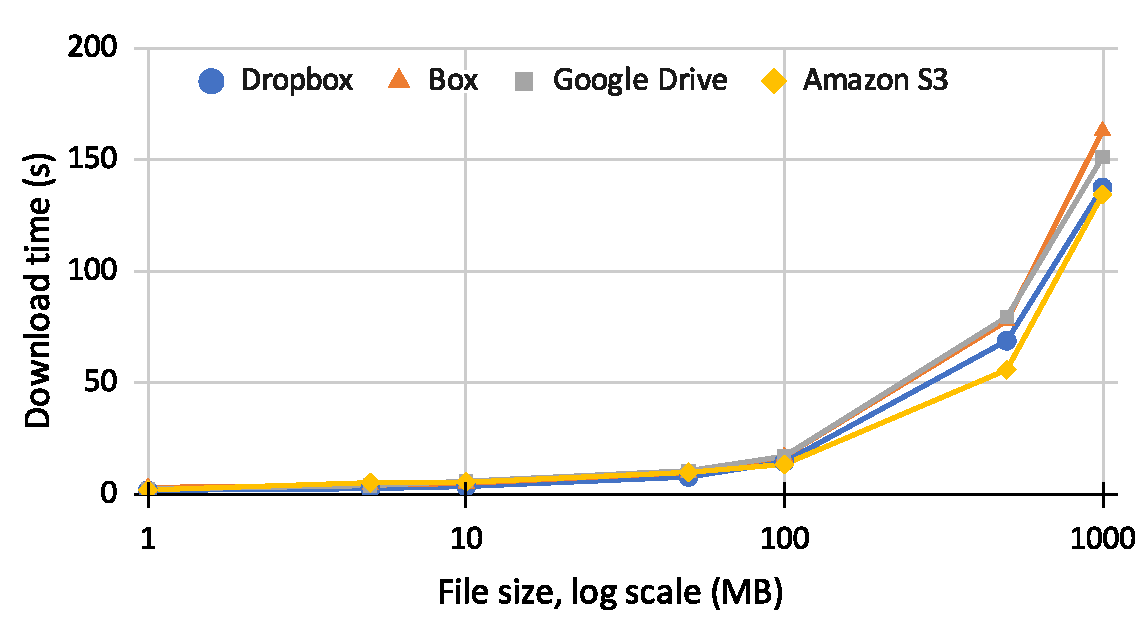
\includegraphics[scale=0.6]{images/download_log_chart}
    \caption{\label{fig:download_log_duration}Download Duration (log scale)}
\end{figure}

\section{Deletion Duration}
The results shown in figure \ref{fig:deletion_duration} and \ref{fig:deletion_log_duration} make it clear that all services perform nearly identically when it comes to deletion duration. Regardless of the file size, Dropbox, Box and Google Drive all take around 1s to successfully delete a file, with a negligible variation of around 0.5s. Box was consistently slower than all services, but the difference was quite insignificant (usually less than 1s)

\begin{figure} [!h]
    \centering
    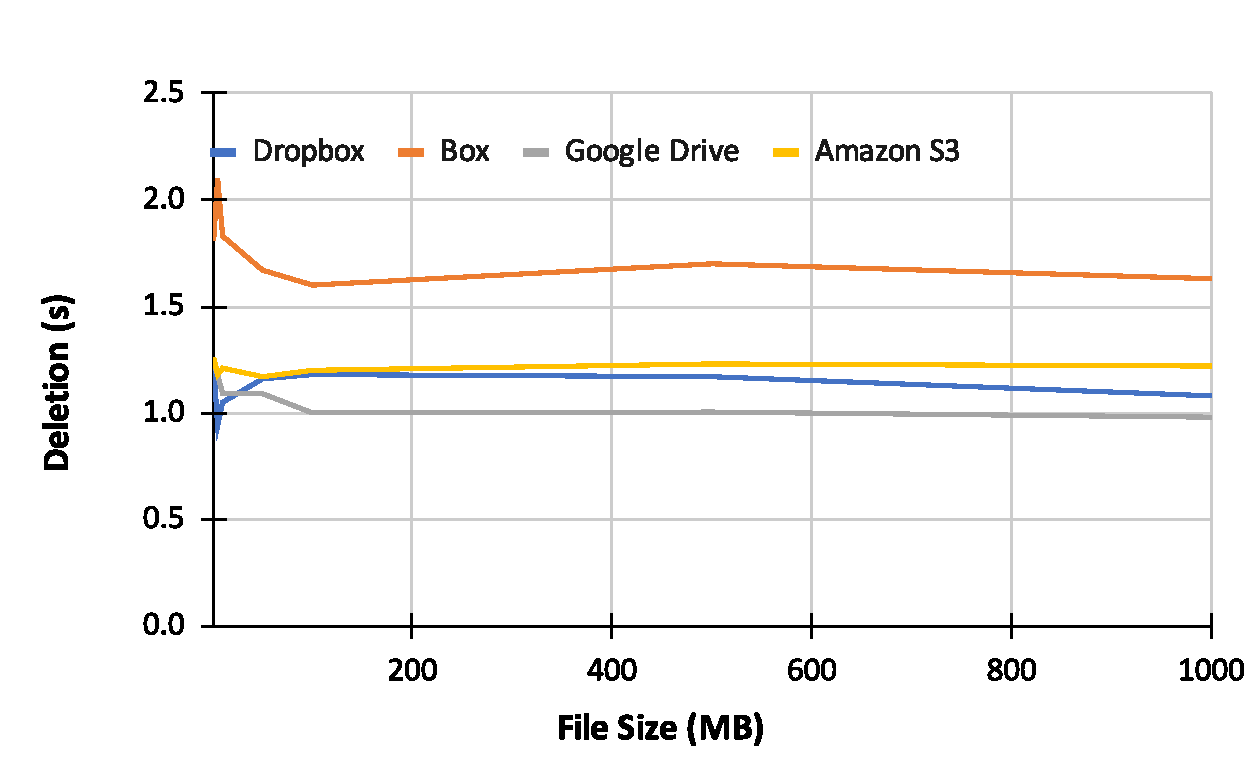
\includegraphics[scale=0.5]{images/deletion_chart}
    \caption{\label{fig:deletion_duration}Deletion Duration}
\end{figure}

\begin{figure} [!h]
    \centering
    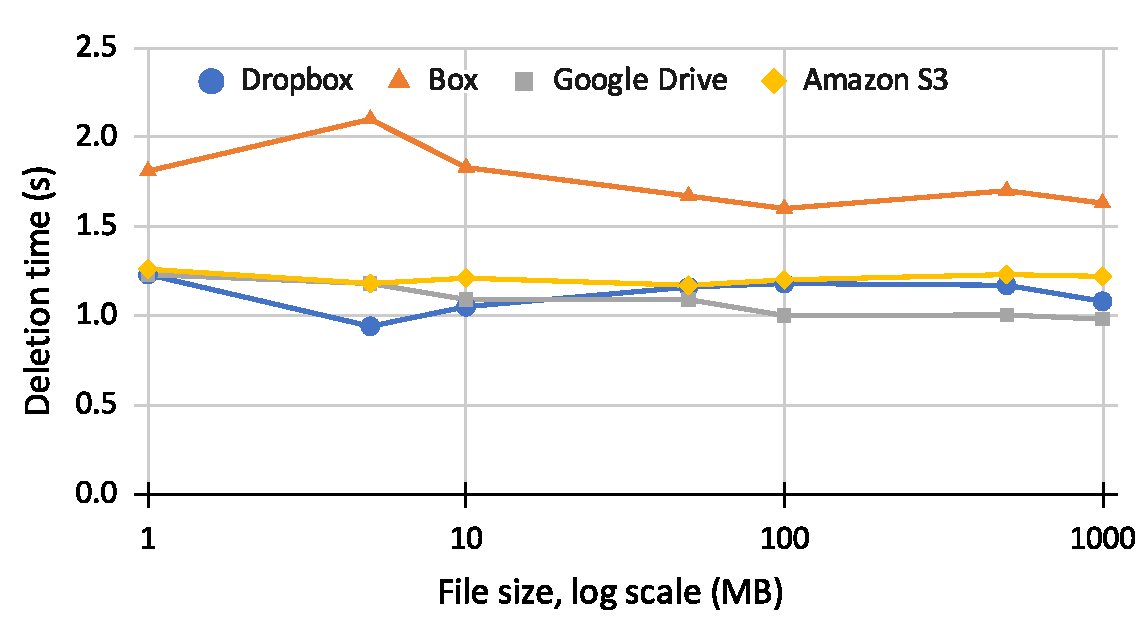
\includegraphics[scale=0.5]{images/deletion_log_chart}
    \caption{\label{fig:deletion_log_duration}Deletion Duration (log scale)}
\end{figure}